%
\hsection{Downloading the Example Codes}%
%
\begin{figure}%
\centering%
%
\subfloat[][%
We use a webbrowser to visit the website~\expandafter\url{\databasesCodeRepo}. %
On the website, we click on the green \menu{Code} menu.%
\label{fig:examplesBrowser1website}%
]{\parbox[t]{0.9999\linewidth}{\centering\tightbox{%
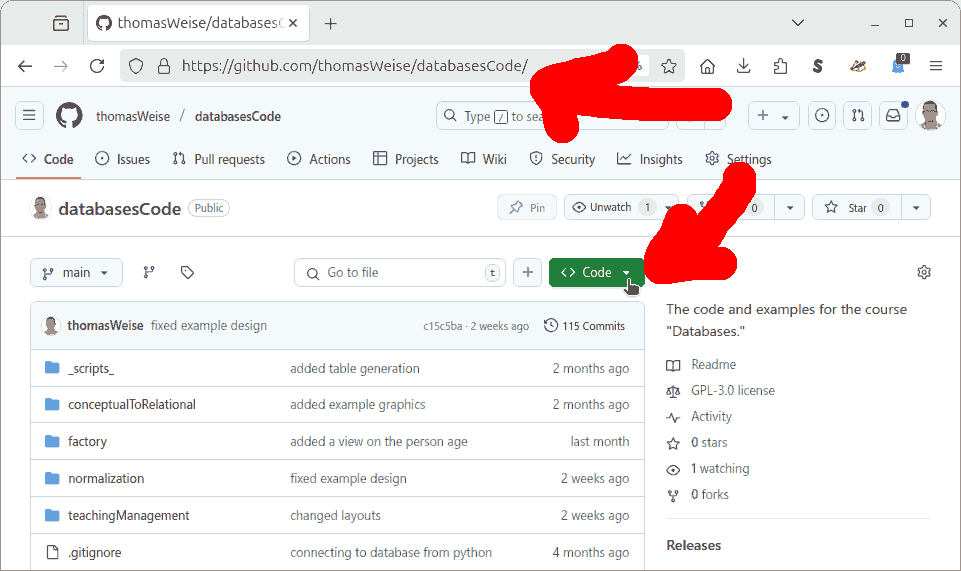
\includegraphics[width=0.7\linewidth]{\currentDir/examplesBrowser1website}}}}%
%
\floatRowSep%
%
\subfloat[][%
A small popup-menu appears, where we click on~\menu{Download ZIP}.%
\label{fig:examplesBrowser2beginDownload}%
]{\parbox[t]{0.9999\linewidth}{\centering\tightbox{%
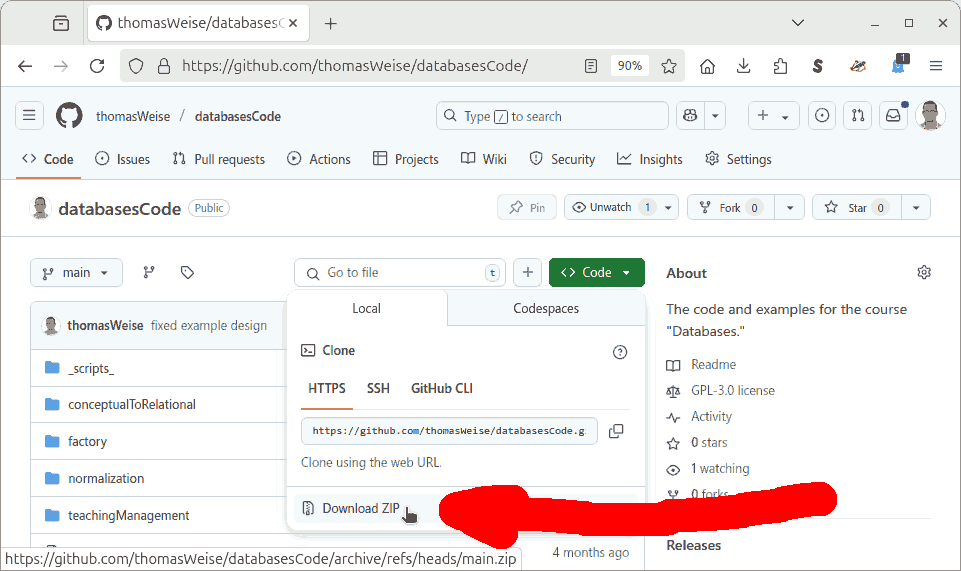
\includegraphics[width=0.7\linewidth]{\currentDir/examplesBrowser2beginDownload}}}}%
%
\label{fig:examplesBrowser:A}%
\caption{Downloading the examples from this book.}%
\end{figure}%
%
\begin{figure}%
\centering%
%
\subfloat[][%
Once the file is downloaded, we open it.%
\label{fig:examplesBrowser3downloaded}%
]{\parbox[t]{0.9999\linewidth}{\centering\tightbox{%
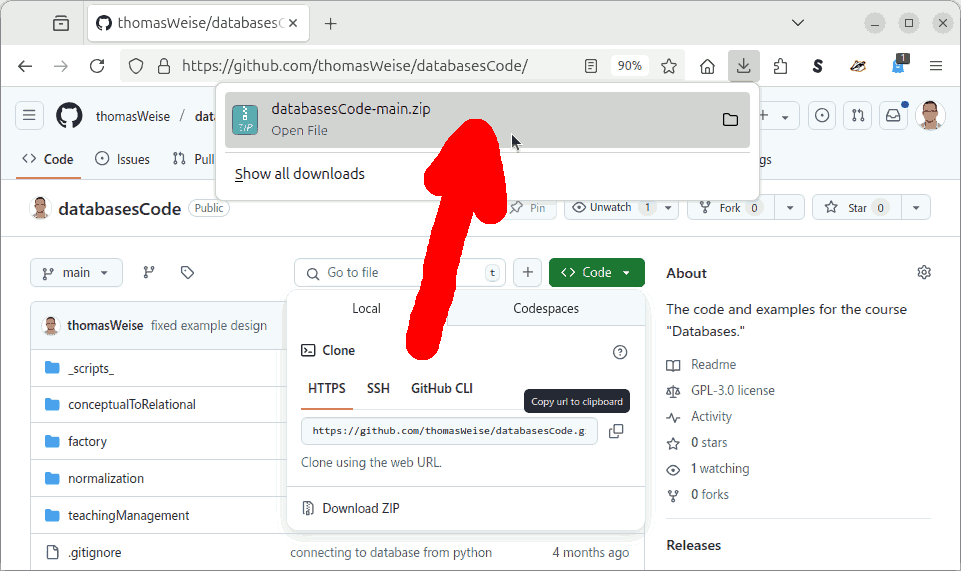
\includegraphics[width=0.7\linewidth]{\currentDir/examplesBrowser3downloaded}}}}%
%
\floatRowSep%
%
\subfloat[][%
In the opened archive, we can find \emph{all} the examples of this book. %
In folder \textil{factory}, we find the simple factory example.
\label{fig:examplesBrowser4opened}%
]{\parbox[t]{0.9999\linewidth}{\centering\tightbox{%
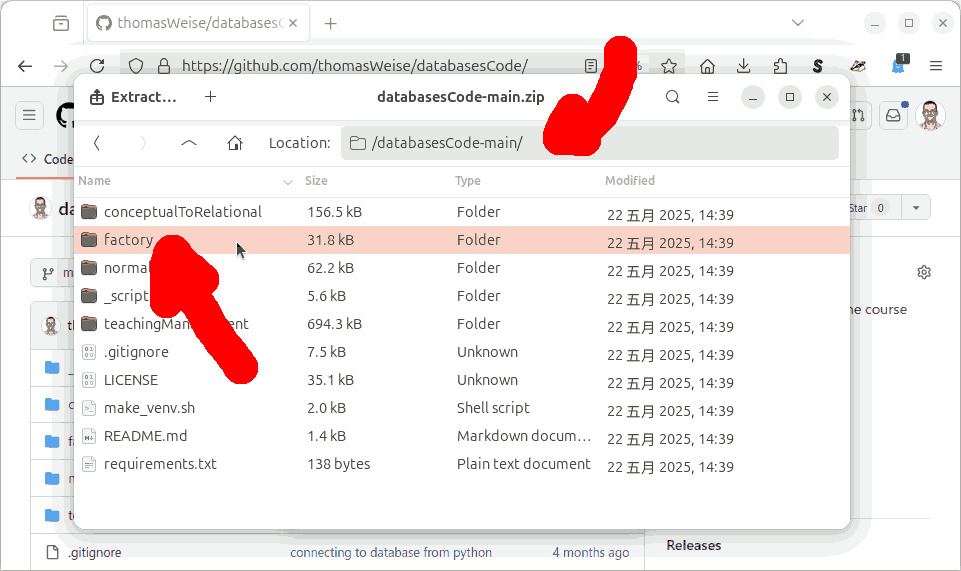
\includegraphics[width=0.7\linewidth]{\currentDir/examplesBrowser4opened}}}}%
%
\label{fig:examplesBrowser:B}%
\caption{Downloading the examples from this book.~(Continued)}%
\end{figure}%
%
In the previous two sections, we discussed how a new \db\ user and how a new \db\ can be created, using \sql\ on the \postgresql\ \dbms\ \pgls{server} via the \psql~\pgls{client}.
There, we mentioned that there are two ways to do that with \psql:
We can either type in the commands manually in an interactive session.
Or we can tell \psql\ to execute an \sql~script on the \pgls{server}.

The latter way is maybe more convenient.
For all the examples that follow in this book, we provide such scripts.
So you do not need to type in the examples from the book.

All these examples are provided in the repository~\texttt{\databasesCodeRepoName} on \github.
You can either clone this repository using~\git, which is explained in our book \citetitle{programmingWithPython}~\cite{programmingWithPython}.
Our you can just visit this repository at \expandafter\url{\databasesCodeRepo} with your webbrowser and download the files.
This is illustrated in \cref{fig:examplesBrowser:A}.

As shown in \cref{fig:examplesBrowser1website}, you would use your  webbrowser to visit the website~\expandafter\url{\databasesCodeRepo}.
Once the website has loaded, you click on the green \menu{Code} menu.
Then, in \cref{fig:examplesBrowser2beginDownload}, a small popup-menu appears, where you click on~\menu{Download ZIP}.
This will download a so-called ZIP-archive, i.e., a file that contains a compressed folder structure with all files in our examples repository.
After the download completes, as illustrated in \cref{fig:examplesBrowser3downloaded}, you then can open the archive.
In the opened archive, you can find \emph{all} the examples of this book in a folder called \textil{databasesCode-main}.
This folder contains another folder called \textil{factory}, where you can find all the files belonging to our present example, as shown in \cref{fig:examplesBrowser4opened}.

Additionally, each source code listing has a headline containing some text like~\inQuotes{(stored in file \textil{myfile};.}
\textil{myfile} then is a clickable link that would take you directly to the file on \github.%
%
\FloatBarrier%
\endhsection%
%
